\documentclass{standalone}
\usepackage{tikz}
\usetikzlibrary{decorations.pathmorphing, arrows.meta}

\begin{document}

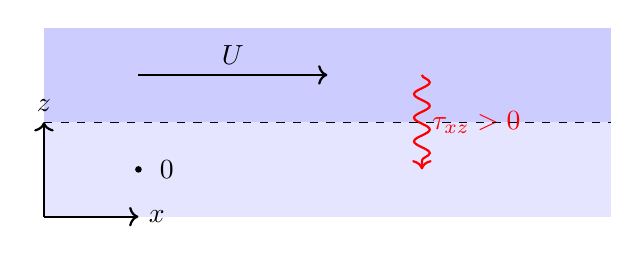
\begin{tikzpicture}[scale=1.2]

  % Draw top and bottom layers
  \fill[blue!20] (0,1) rectangle (6,2); % Top layer
  \fill[blue!10] (0,0) rectangle (6,1); % Bottom layer

  % x and z axes
  \draw[->, thick] (0,0) -- (1.0,0) node[right] {$x$};
  \draw[->, thick] (0,0) -- (0,1.0) node[above] {$z$};
  % Velocity arrow in top layer
  \draw[->, thick] (1,1.5) -- (3,1.5) node[midway, above] {$U$};

  % Velocity arrow in bottom layer (zero velocity, optional small arrow or just a dot)
  \fill (1,0.5) circle (1pt);
  \node at (1.3,0.5) {$0$};

  % Squiggly arrow for momentum transfer
  \draw[->, decorate, decoration={snake, amplitude=1mm, segment length=3mm}, thick, red]
    (4,1.5) -- (4,0.5) node[midway, right] {$\tau_{xz} > 0$};

  % Optional dashed line separating the layers
  \draw[dashed] (0,1) -- (6,1);

\end{tikzpicture}

\end{document}
